\documentclass[aspectratio=169]{beamer}
\usepackage{cmap}
\usepackage{xfrac}
\usepackage[utf8]{inputenc}
\usepackage[T2A]{fontenc}
\usepackage[russian]{babel}
\usepackage{graphicx}
\usepackage{xcolor}
\usepackage{amsmath}
\DeclareMathOperator*{\argmax}{arg\,max}
\DeclareMathOperator*{\argmin}{arg\,min}


\usetheme{Berlin}

\title[Моделирование количества подвижных единиц в сходе с рельсов]{Моделирование количества подвижных единиц грузового поезда в сходе с рельсов на основе метода максимального правдоподобия}
\author[Е.В.Королёв \and А.Н.Игнатов]{Работу выполнил: Королёв Егор Владимирович, студент группы М8О-401Б-18 \and Научный руководитель: Игнатов Алексей Николаевич, к.ф.-м.н., доцент кафедры 804 МАИ}
\institute[НИУ МАИ]{Московский авиационный институт (НИУ)}
\date{}

\newcommand{\norm}[1]{\left\lVert#1\right\rVert}
\definecolor{myBlue}{RGB}{0, 128, 0}
\definecolor{myGreen}{RGB}{1, 4, 255}

\begin{document}
    \begin{frame}
        \maketitle
    \end{frame}


    \section{Введение}
    \begin{frame}{1. Введение}
        \begin{block}{Проблема}
            Периодически на ЖД путях происходят сходы или крушения. Последствия схода могут привести к экологическим, экономическим и логистическим проблемам. В РФ в среднем происходит сход или крушение раз в 5.5 дней.
        \end{block}
    
        \begin{block}{Задача}
            По имеющемуся набору данных необходимо построить предсказательную модель количества сошедших подвижных единиц в составе.
        \end{block}
    \end{frame}

    \begin{frame}{2. Введение}
        \begin{block}{Причина схода}
            Самая частая причина схода -- излом боковой рамы
        \end{block}
    
        \centering
        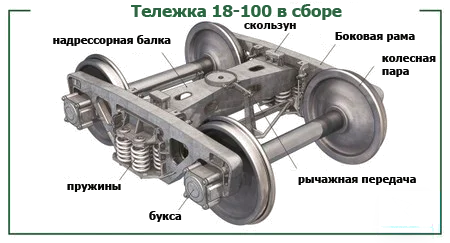
\includegraphics[width=0.55\linewidth]{src/тележка_в_сборе.png}
        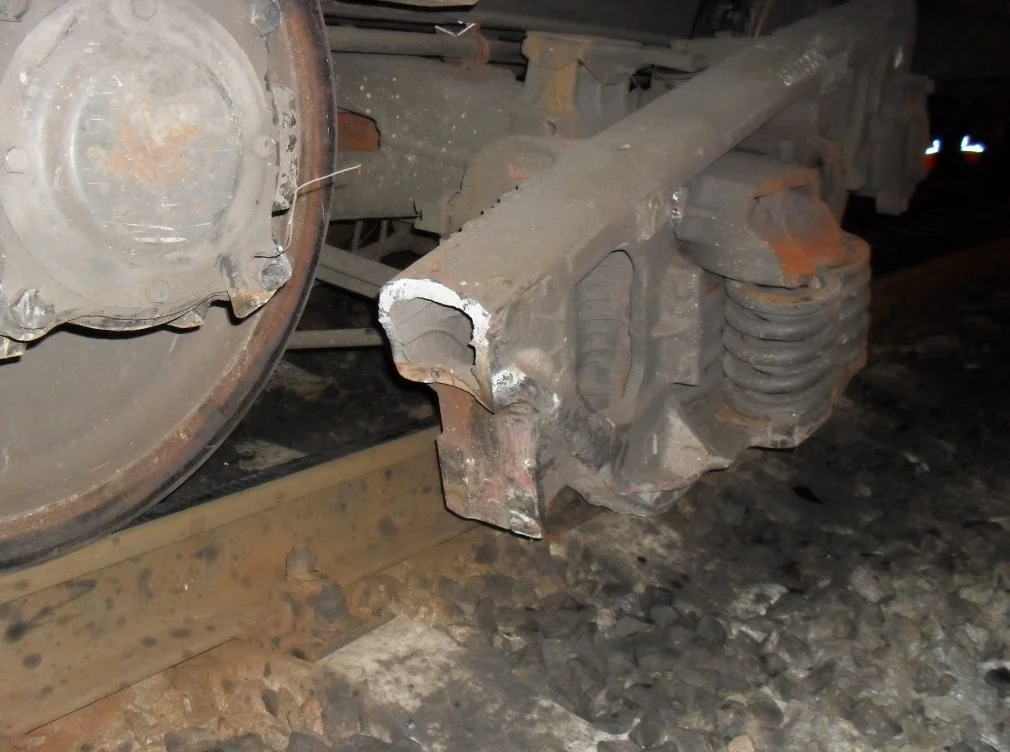
\includegraphics[width=0.4\linewidth]{src/излом.png}
    \end{frame}

    \begin{frame}{3. Введение}
        \centering
        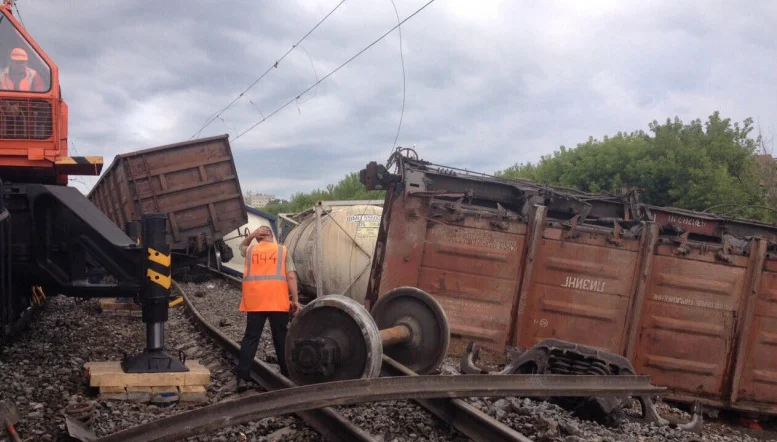
\includegraphics[width=0.7\linewidth]{src/крушение.png}
    \end{frame}

    \begin{frame}{4. Введение}
        \begin{block}{Некоторые обозначения}
            \begin{itemize}
                \item $n$ -- мощность выборки;
                \item $r$ -- количество параметров в обучаемой модели;
                \item $\xi$ -- СВ, характеризующая количество подвижных единиц в сходе;
                \item $\eta = \xi -1$;
                \item $\theta$ -- вектор обучаемых параметров;
                \item $AIC_c = 2r - 2\ln(L) + \frac{2r^2 + 2r}{n - r - 1}$ -- скорректированный критерий Акаике;
                \item $L$ -- значение функции правдоподобия для обученной модели.
            \end{itemize}
        \end{block}
    \end{frame}


    \begin{frame}{5. Введение}
        \begin{block}{Некоторые обозначения}
            \begin{itemize}
                %\item $x$ -- вектор признаков объекта;
                %\item $y$ -- целевая переменная; количество подвижных единиц в сходе минус 1;
                \item $x_i$ -- вектор признаков $i$-го происшествия;
                \item $y_i$ -- количество подвижных единиц в сходе $i$-го происшествия;
                \item $L_{best}$ -- значение функции правдоподобия у наилучшей модели по $AIC_c$;
                \item $L_{trivial}$ -- значение функции правдоподобия для тривиальной модели.
            \end{itemize}
        \end{block}
    \end{frame}


    \section{Предварительный анализ данных}
    \begin{frame}{1. Описание признаков}
        \centering
        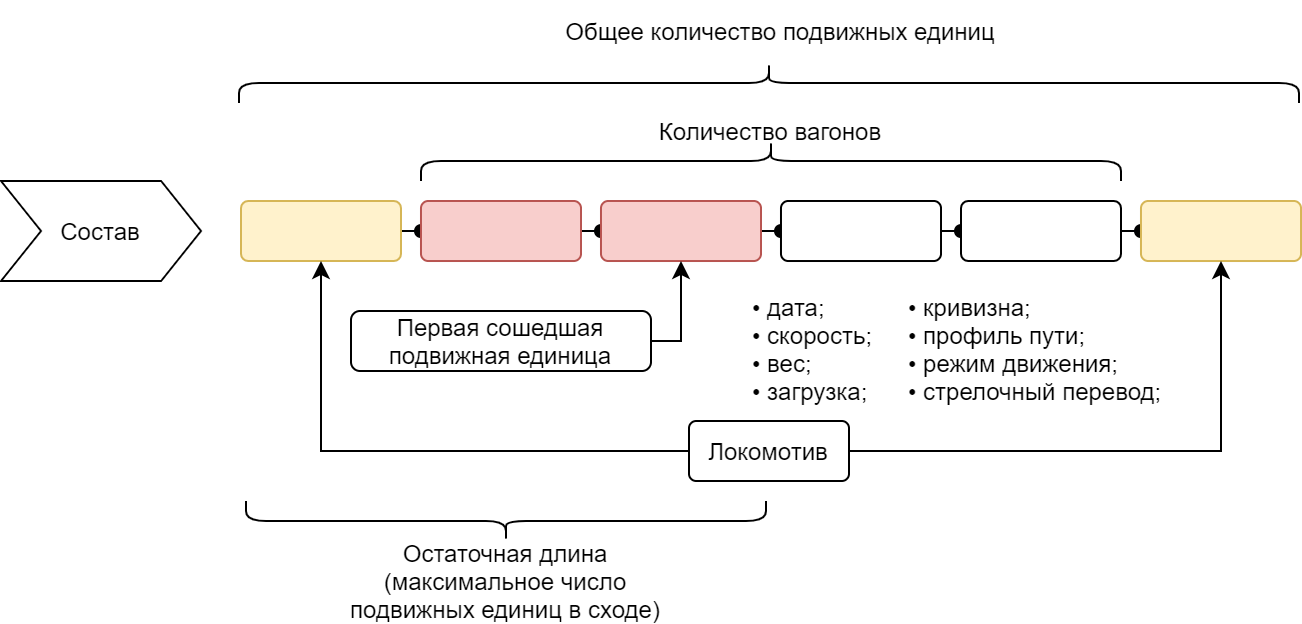
\includegraphics[width=0.8\linewidth]{src/train.png}
    \end{frame}


    \begin{frame}{2. Описание признаков}
        \begin{block}{Разреженность данных}
            \begin{itemize}
                \item мощность выборки $n = 56$;
                \item признак 'Режим движения' имеет $23$ пропусков ($41\%$);
                \item признак 'Профиль пути' имеет $12$ пропусков ($21\%$);
                \item признак 'Кривизна' имеет $10$ пропусков ($17\%$);
            \end{itemize}
        \end{block}
    \end{frame}


    \begin{frame}{3. Корреляция признаков}
        \centering
        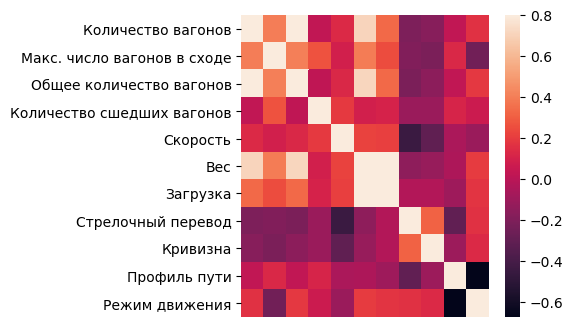
\includegraphics[width=1.3\textheight]{src/corr_plot.png}
    \end{frame}


    \begin{frame}{4. Конструирование признаков}
        \begin{block}{Введение новых признаков}
            \begin{itemize}
                \item $f_1 = $ профиль пути $\cdot$ макс. число вагонов в сходе;
                \item $f_2 = 1 - \frac{\text{макс. число вагонов в сходе}}{\text{общее кол-во вагонов}}$;
                \item $f_3 = $ скорость $\cdot$ загрузка;
            \end{itemize}
        \end{block}
    
        \begin{center}
            \begin{tabular}{|l|c|c|c|c|}
                \hline
                & target & $f_1$ & $f_2$ & $f_3$ \\ \hline
                target & 1.0       & 0.101  & -0.286 & 0.198  \\ \hline
                $f_1$  & 0.101  & 1.0       & -0.086 & -0.228 \\ \hline
                $f_2$  & -0.286 & -0.086 & 1.0       & -0.124 \\ \hline
                $f_3$  & 0.198  & -0.228 & -0.124 & 1.0       \\ \hline
            \end{tabular}
        \end{center}
    \end{frame}


    \begin{frame}{5. Оценка функции вероятности $P(\xi = l)$}
        \centering
        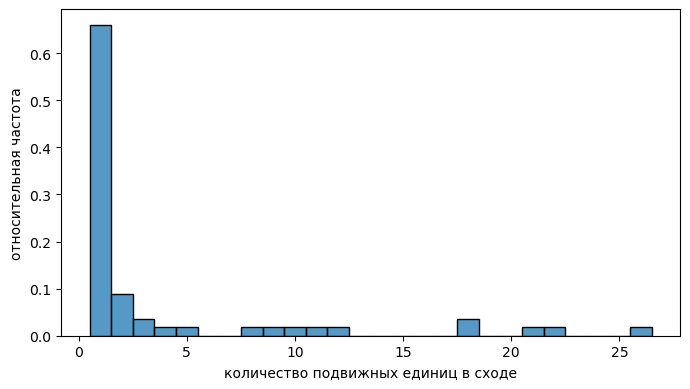
\includegraphics[width=1.3\textheight]{src/KDE.png}
    \end{frame}


    \section{Построение моделей}    
    \begin{frame}{1. Пуассоновская регрессия}
        \begin{block}{Функция вероятности}
            $$P(\eta = k) = \dfrac{\lambda^k}{k!}e^{-\lambda}$$
        \end{block}
        
        \begin{block}{Функция логарифмического правдоподобия}
            $$\ln(L(\theta, x, y)) = \sum\limits_{i=1}^{n} \left( -\lambda(\theta, x_i) + (y_i - 1) \ln(\lambda(\theta, x_i)) - \ln((y_i - 1)!) \right),$$
            
            где $x = col(x_1, x_2, \ldots, x_n), y = col(y_1, y_2, \ldots, y_n)$.
        \end{block}
    \end{frame}


    \begin{frame}{2. Определение функций $\lambda(\theta, x)$}
        \begin{enumerate}
            \item $\lambda_1(\theta, x) = e^{\left\langle \theta, x\right\rangle }$;
            \item $\lambda_2(\theta, x) = e^{-(\left\langle\theta, x\right\rangle)^2}$;
            \item $\lambda_3(\theta, x) = \sqrt{|5^2 - (\left\langle\theta, x\right\rangle - 5)^2|} + 1$;
            \item $\lambda_4(\theta, x) = (\left\langle\theta, x\right\rangle - 1)^2$;
            \item $\lambda_5(\theta, x) = \frac{1}{1 + (\left\langle\theta, x\right\rangle)^2}$;
            \item $\lambda_6(\theta, x) = \left\langle\theta, x\right\rangle (\frac{\pi}{2} + \arctan(\left\langle\theta, x\right\rangle)) + 1$;
            \item $\lambda_7(\theta, x) = \ln(1 + (\left\langle\theta, x\right\rangle )^2) + 1$.
        \end{enumerate}
    \end{frame}


    \begin{frame}{3. Геометрическая регрессия}
        \begin{block}{Функция вероятности}
            $$P(\eta = k) = (1-p)^k p$$
        \end{block}
        
        \begin{block}{Функция логарифмического правдоподобия}
            $$\ln(L(\theta, x, y)) = \sum\limits_{i = 1}^n ( (y_i - 1) \ln(1 - p(\theta, x_i)) + \ln(p(\theta, x_i)) ),$$
            
            где $x = col(x_1, x_2, \ldots, x_n), y = col(y_1, y_2, \ldots, y_n)$.
        \end{block}        
    \end{frame}

    
    \begin{frame}{4. Определение функций $p(\theta, x)$}
        \begin{enumerate}
            \item $p_1(\theta, x) = e^{\left\langle \theta, x \right\rangle }$;
            \item $p_2(\theta, x) = e^{-(\left\langle\theta, x\right\rangle)^2}$;
            \item $p_3(\theta, x) = \frac{1}{1+e^{-\left\langle\theta, x\right\rangle}}$;
            \item $p_4(\theta, x) = \frac{1}{1 + (\left\langle\theta, x\right\rangle)^2}$;
            \item $p_5(\theta, x) = \left\langle \theta, x\right\rangle (\frac{\pi}{2} + \arctan(\left\langle \theta, x\right\rangle)) + 1$.
        \end{enumerate}
    \end{frame}


    \begin{frame}{5. Признаковые пространства}
        \begin{enumerate}
            \item $features_1:$ (кривизна);
            \item $features_2:$ (кривизна, профиль пути);
            \item $features_3:$ (кривизна, профиль пути $\cdot$ макс. число вагонов в сходе);
            \item $features_4:$ (кривизна, $1 - \frac{\text{макс. число вагонов в сходе}}{\text{общее кол-во вагонов}}$);
            \item $features_5:$ (кривизна, профиль пути, скорость $\cdot$ загрузка);
            \item $features_6:$ (кривизна, профиль пути, скорость $\cdot$ загрузка,\\ $1 - \frac{\text{макс. число вагонов в сходе}}{\text{общее кол-во вагонов}}$);
            \item $features_7:$ (кривизна, скорость $\cdot$ загрузка, $1 - \frac{\text{макс. число вагонов в сходе}}{\text{общее кол-во вагонов}}$);
            \item $features_8:$ (скорость $\cdot$ загрузка, $1 - \frac{\text{макс. число вагонов в сходе}}{\text{общее кол-во вагонов}}$).
            \newline
        \end{enumerate}
    \end{frame}

    
    \section{Численный эксперимент}
    \begin{frame}{1. Программная реализация ММП}
        \begin{block}{Конструктор класса}
            \textcolor{myGreen}{def} \textcolor{myBlue}{MLM}(log\_likelihood\_fun,\\
            \begin{tabular}{p{1cm}l}
                & optim\_method, borders,\\
                & predict\_fun, link\_fun,\\
                & features, target, df)
            \end{tabular}
        \end{block}
    \end{frame}
    
    
    \begin{frame}{2. Численный эксперимент}
        \scriptsize
        \begin{block}{Пуассоновская регрессия}
            \begin{itemize}
                \item наилучшая модель (по признаковым пространствам и функциям связи): $(\lambda_1, features_6)$. $AIC_c = 356.87,~~\hat\theta=(0.92, -105.33, 34.34, 0.02, -2.24)$, $\frac{\ln(L_{best})}{\ln(L_{trivial})} = 0.62$;
                \item $AIC_c \in [356.87, 567.74]$;
                \item в условиях (а) $\argmax_k \hat{P}(\xi = k)$ $ = 2$.
            \end{itemize}
        \end{block}
    
        \begin{block}{Геометрическая регрессия}
            \begin{itemize}
                \item наилучшая модель: $(p_4, features_6)$. $AIC_c = 153.65,~~\hat\theta=(-2.01, 29.36, 226.20, -0.03, 3.85)$, $\frac{\ln(L_{best})}{\ln(L_{trivial})} = 0.57$;
                \item $AIC_c \in [153.65, 918.43]$;
                \item в условиях (а) $\argmax_k \widetilde{P}(\xi = k)$ $ = 1$.
            \end{itemize}
        \end{block}
    
         (а). профиль пути $ = 0.001555$, кривизна$=0.001875$, скорость$=67$, загрузка$=0.87$, макс.число вагонов в сходе$=21$, общее кол-во вагонов$=67$
        
        \normalsize
    \end{frame}


    \section{Веб сервис}
    \begin{frame}{1. Демонстрация работы}
        \centering
        
\includegraphics[width=2.05\textheight]{src/web/1.jpg}
    \end{frame}
    \begin{frame}{2. Демонстрация работы}
        \centering
        
\includegraphics[width=2.05\textheight]{src/web/2.jpg}
    \end{frame}
    \begin{frame}{3. Демонстрация работы}
        \centering
        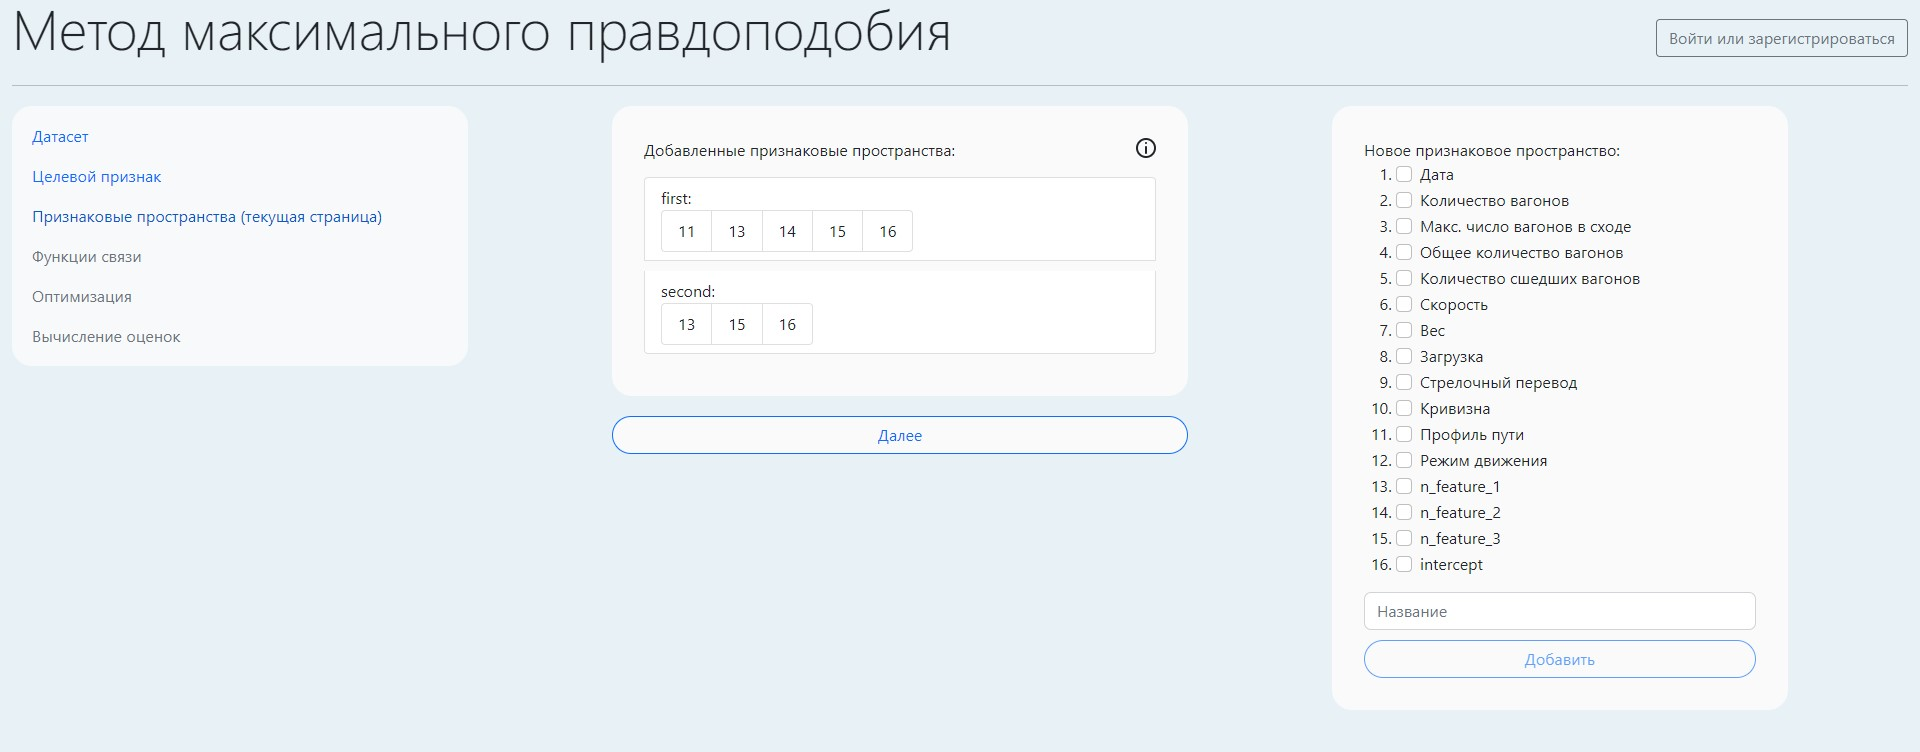
\includegraphics[width=1.75\textheight]{src/web/3.jpg}
    \end{frame}
    \begin{frame}{4. Демонстрация работы}
        \centering
        
\includegraphics[width=2.0\textheight]{src/web/4.jpg}
    \end{frame}
    \begin{frame}{5. Демонстрация работы}
        \centering
        
\includegraphics[width=2.05\textheight]{src/web/5.jpg}
    \end{frame}
    \begin{frame}{6. Демонстрация работы}
        \centering
        
\includegraphics[width=2.05\textheight]{src/web/6.jpg}
    \end{frame}
    \begin{frame}{7. Демонстрация работы}
        \centering
        
\includegraphics[width=2.05\textheight]{src/web/7.jpg}
    \end{frame}
    
    \begin{frame}{8. Схема приложения}
        \centering
        
\includegraphics[width=2.0\textheight]{src/схема_приложения.png}
    \end{frame}

    \section{Заключение}
    \begin{frame}{Заключение}
        \begin{block}{}
            Были построены предсказательные модели числа сошедших подвижных единиц. Их можно разделить на 2 класса: модели пуассоновской регрессии и модели геом. регрессии. Для каждого класса были рассмотрены различные функции связи и признаковые пространства. Были проведены численные эксперименты.
        \end{block}
    
        \begin{block}{}
            Был написан веб-сервис, реализующий метод максимального правдоподобия. Сервис позволяет задать собственный набор данных, целевой признак и его распределение, указать признаковые пространства, функции связи, а также выбрать один из методов оптимизации. Скачать результаты вычислений можно в нескольких форматах.
        \end{block}
    \end{frame}
    
    \begin{frame}{}
        \centering
        \Huge
        Спасибо за внимание!
    \end{frame}

    \begin{frame}{Список литературы}
        \begin{thebibliography}{00}
            \bibitem{Ignatov:functional_dependence} Замышляев А.М., Игнатов А.Н., Кибзун А.И., Новожилов Е.О. Функциональная зависимость между количеством вагонов в сходе из-за неисправностей вагонов или пути и факторами движения // Надежность. -- 2018. -- С.1-15.
        \end{thebibliography}
    \end{frame}

\end{document}

